\section{Loop in Tikz}
\begin{frame}{Use of Loop in Tikz}
\begin{figure}
    \centering
    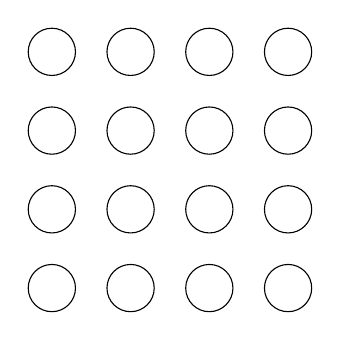
\begin{tikzpicture}
    \foreach \x in {1,2,3,4}
    {\foreach \y in {1,2,3,4}
        {\draw (\x,\y) circle [radius=0.3];
        };
    }
    \end{tikzpicture}
    \caption{Use of Loop}
    \label{fig:loop}
\end{figure}
    
\end{frame}

\begin{frame}{Use of Loop in Tikz continue...}
\begin{figure}
    \centering
    \begin{tikzpicture}
    \draw[thick, ->](0,0)  -- (6,0) node[anchor = west] {x axis};
    \draw[thick, ->] (0,0) -- (0,6) node[anchor = north east] {y axis};
    \foreach \i\j\k in {1/A/0.5,2/B/1,3/C/1.5,4/D/2,5/E/2.5,6/F/3}
    {
        %\draw (0,0) circle [radius=\k];
        \node[draw,shape=circle] at (\i,2){\j};
        \pause
    }
 
    \end{tikzpicture}
    \caption{Fig 2}
\end{figure}
    
\end{frame}
